\documentclass{report}
% PACKAGES %
\usepackage[english]{} % Sets the language
\usepackage[margin=2cm]{geometry} % Sets the margin size
\usepackage{fancyhdr} % Allows creation of headers
\usepackage{graphicx} % Enhanced package for including graphics/figures
\usepackage{float} % Allows figures and tables to be floats
\usepackage{amsmath} % Enhanced math package prepared by the American Mathematical Society
\usepackage{amssymb} % AMS symbols package
\usepackage{mathrsfs}% More math symbols
\usepackage{bm} % Allows you to use \bm{} to make any symbol bold
\usepackage{bbold} % Allows more bold characters
\usepackage{verbatim} % Allows you to include code snippets
\usepackage{setspace} % Allows you to change the spacing between lines at different points in the document
\usepackage{parskip} % Allows you alter the spacing between paragraphs
\usepackage[normalem]{ulem} % Allows underlining to wrap multiple lines
\usepackage{multicol} % Allows text division into multiple columns
\usepackage{units} % Allows fractions to be expressed diagonally instead of vertically
\usepackage{booktabs,multirow,multirow} % Gives extra table functionality
\usepackage{hyperref} % Allows hyperlinks in the document
\usepackage{rotating} % Allows tables to be rotated

\newcommand{\tab}{\-\hspace{1.5cm}}

% Set path to figure image files
\graphicspath{ {"/Users/mitch/Documents/Cal/2 - 2017 Spring/COMPSCI 289A - Intro to Machine Learning/HW03/Figures/"} }

% Create a header w/ Name & Date
\pagestyle{fancy}
\rhead{\textbf{Mitch Negus} 3032146443}

\begin{document}
\thispagestyle{empty}

{\bf {\large {COMPSCI 289A} Homework {3} \hfill Mitch Negus\\
		2/27/2017 						\hfill	3032146443}}\\\\


%%%%%%%%%%%%%%%%%%%%%%%%%%%%%%%%%% PROBLEM 1 %%%%%%%%%%%%%%%%%%%%%%%%%%%%%%%%%%
\section*{Problem 1}

\subsection*{\textit{a.})}

$X$ and $Y$ are independent if $P(X=x \cap Y=y) = P(X=x)P(Y=y)$. Given that $P(X=0 \cap Y=0) = 0$ since $X$ and $Y$ are never both zero, we find
$$ P(X=0 \cap Y=0) \neq P(X=0)P(Y=0) $$
$$ 0 \neq 0.5 \cdot 0.5 = 0.25 .$$
$X$ and $Y$ are \underline{not} independent.

$X$ and $Y$ are uncorrelated if $E[XY] = E[X]E[Y]$. By using the definition of the expectation value, we can state
$$ E[XY] = \int{xy f(x,y) \;dx\,dy} $$ 
Since either $X=0$ or $Y=0$, 
$$ E[XY] = \int{(0) f(x,y) \;dx\,dy} = 0 $$
Similarly
$$ E[X]E[Y] = \int{x f(x,y) \;dx\,dy} \int{y f(x,y) \;dx\,dy} $$
and, when solved for the discrete values for $X$ and $Y$, is
$$ E[X]E[Y] = \left( (1)(0.25) + (-1)(0.25) \right) \left( (1)(0.25) + (-1)(0.25) \right) $$
$$ E[X]E[Y] = 0 $$
$$\boxed{ E[XY] = E[X]E[Y] = 0 }.$$


\subsection*{\textit{b.})}
We are given that 
\begin{multicols}{3}
$ P(B=0) = \frac{1}{2} $ \\
$ P(B=1) = \frac{1}{2} $ \\

$ P(C=0) = \frac{1}{2} $ \\
$ P(C=1) = \frac{1}{2} $ \\

$ P(D=0) = \frac{1}{2} $ \\
$ P(D=1) = \frac{1}{2} $ \\
\end{multicols}
and that
\begin{multicols}{3}
$ P(X) = P(B \oplus C) $ \\
$ P(X) = P(B)P(\bar{C}) + P(\bar{B})P(C) $\\

$ P(Y) = P(C \oplus D)  $ \\
$ P(Y) = P(C)P(\bar{D}) + P(\bar{C})P(D) $\\

$ P(Z) = P(B \oplus D)  $ \\
$ P(Z) = P(B)P(\bar{D}) + P(\bar{B})P(D) $\\
\end{multicols}

$P(X),P(Y),\text{ and }P(Z)$ are mutually independent if $P(X \cap Y \cap Z) = P(X)P(Y)P(Z)$.
$$ P(X \cap Y \cap Z) = P(X)P(Y)P(Z) $$

By constructing a table (above) showing the 8 unique outcomes, all of equal probability, we can see that each outcome has a probability of 1/8; $P(X \cap Y \cap Z) = 1/8. $
\begin{table}[htbp]
	\centering
	\begin{tabular}{ccc}
		$X$  & $Y$ & $Z$ \\
		\midrule
		0 & 0 & 0 \\
		0 & 0 & 1 \\
		0 & 1 & 0 \\
		0 & 1 & 1 \\
		1 & 0 & 0 \\
		1 & 0 & 1 \\
		1 & 1 & 0 \\
		1 & 1 & 1 \\
		\\
	\end{tabular}%
\end{table}%

Additionally, since
$$ P(X) = P(B)P(\bar{C}) + P(\bar{B})P(C) $$
and if we let the positive case $P(B) = P(B=0) \therefore P(\bar(B)) = P(B=1)$ (and we use a similar convention for $P(C)$ and $P(D)$) then
$$ P(X) = P(B=0)P(C=1) + P(B=1)P(C=0) $$
$$ P(X) = \left(\frac{1}{2}\right)\left(\frac{1}{2}\right) + \left(\frac{1}{2}\right)\left(\frac{1}{2}\right) $$
$$ P(X) = \left(\frac{1}{4}\right) + \left(\frac{1}{4}\right) $$
$$ P(X) = \left(\frac{1}{2}\right). $$
Following the same procedure for $P(Y)$ and $P(Z)$, we find $P(X) = 1/2, P(Y) = 1/2, \text{ and } P(Z) = 1/2$. Then, we can write
$$ P(X)P(Y)P(Z) = \left(\frac{1}{2}\right)^3 $$
$$ P(X)P(Y)P(Z) = \frac{1}{8} $$
and so indeed
$$ P(X \cap Y \cap Z) = P(X)P(Y)P(Z) = \frac{1}{8}. $$
Therefore, we know that $X$, $Y$, and $Z$ are mutually independent (and therefore also pairwise independent). 



\newpage
%%%%%%%%%%%%%%%%%%%%%%%%%%%%%%%%%% PROBLEM 2 %%%%%%%%%%%%%%%%%%%%%%%%%%%%%%%%%%
\section*{Problem 2}

\begin{multicols}{2}

\subsection*{\textit{a.})}
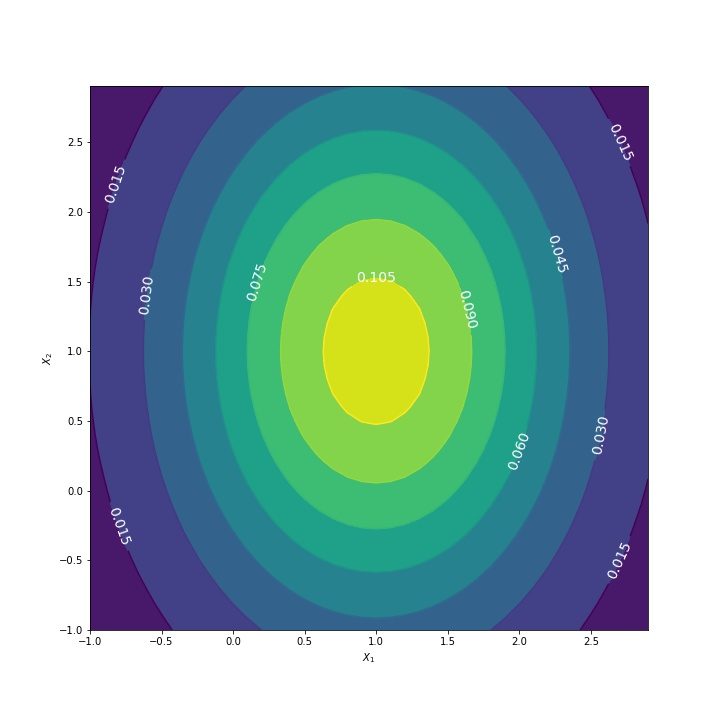
\includegraphics[width=10cm]{HW03_prob2a.jpg}

\subsection*{\textit{b.})}
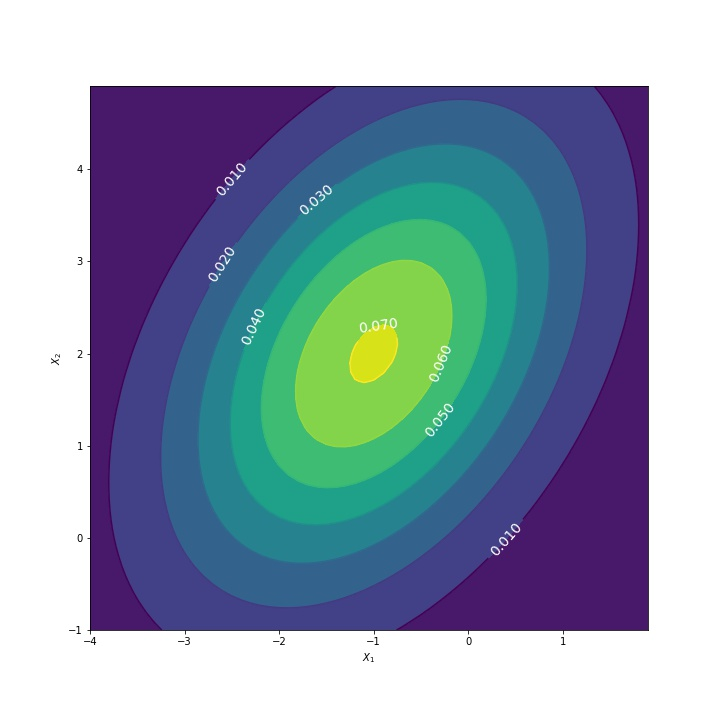
\includegraphics[width=10cm]{HW03_prob2b.jpg}

\subsection*{\textit{c.})}
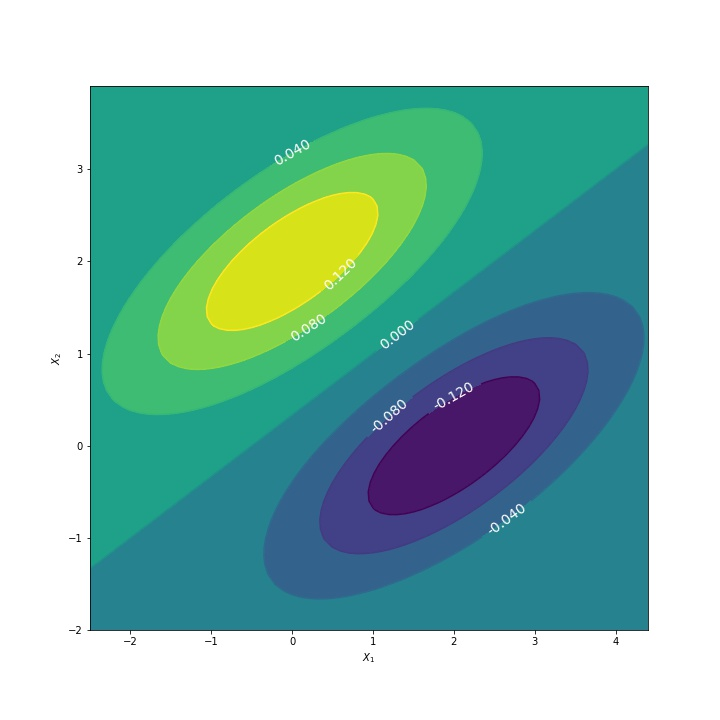
\includegraphics[width=10cm]{HW03_prob2c.jpg}

\subsection*{\textit{d.})}
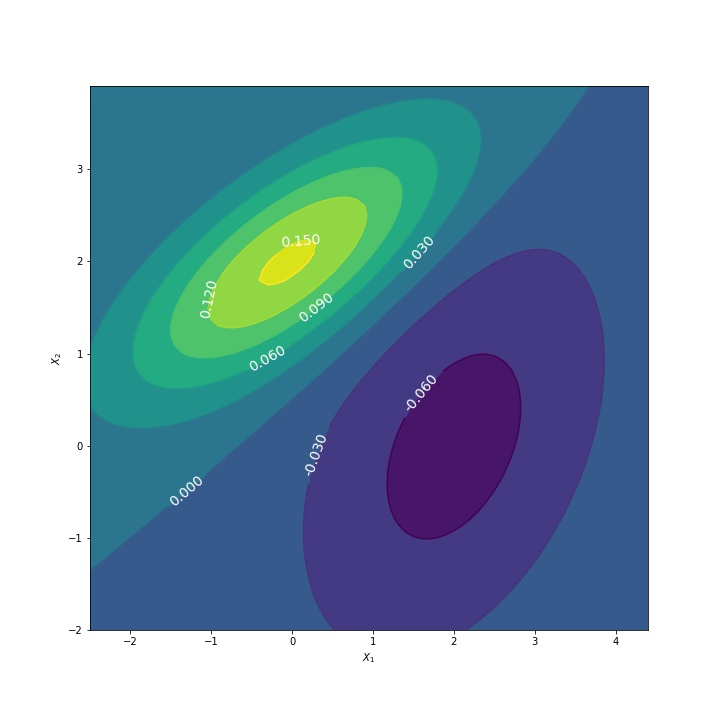
\includegraphics[width=10cm]{HW03_prob2d.jpg}

\subsection*{\textit{e.})}
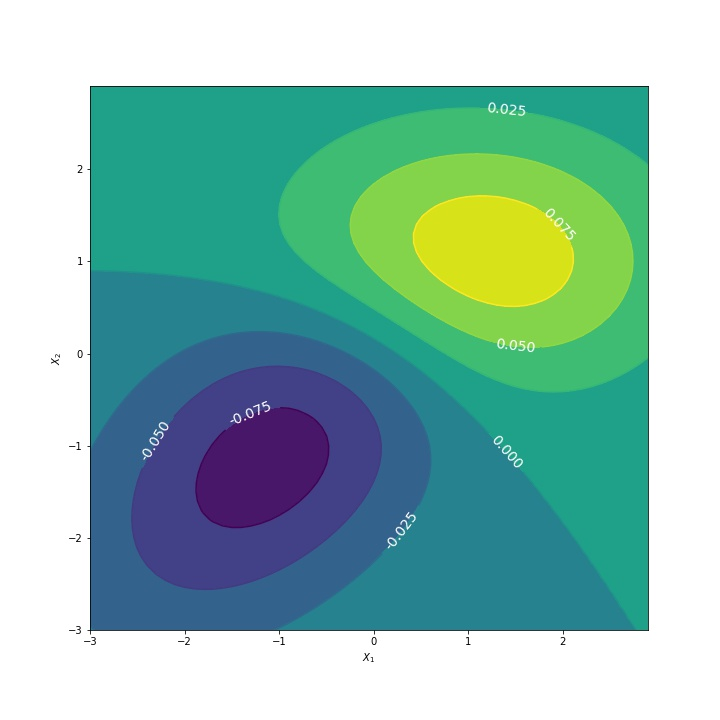
\includegraphics[width=10cm]{HW03_prob2e.jpg}

\end{multicols}



\newpage
%%%%%%%%%%%%%%%%%%%%%%%%%%%%%%%%%% PROBLEM 3 %%%%%%%%%%%%%%%%%%%%%%%%%%%%%%%%%%
\section*{Problem 3}

\begin{multicols}{3}

\subsection*{\textit{a.})} 
 Mean: $\begin{pmatrix} 3.18 \\ 5.09 \end{pmatrix}$\\

\subsection*{\textit{b.})} 
$2 \times 2$ Covariance Matrix:\\
$\begin{pmatrix} 8.49& 4.52 \\
			4.52 & 7.19 \end{pmatrix}$
			
\subsection*{\textit{c.})} 
Eigenvalues: 12.41, 3.27 \\
Eigenvectors: $\begin{pmatrix} 0.76 \\  0.65 \end{pmatrix}$, $\begin{pmatrix} -0.65 \\ 0.76 \end{pmatrix}$\\

\end{multicols}
\-\\
\-\\
\begin{multicols}{2}

\subsection*{\textit{d.})} 
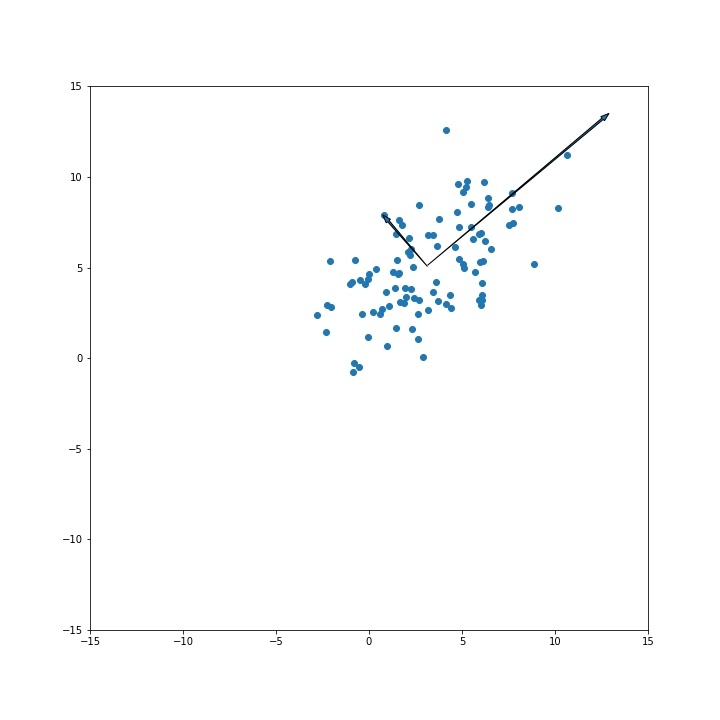
\includegraphics[width=8cm]{HW03_prob3d.jpg}

\subsection*{\textit{e.})} 
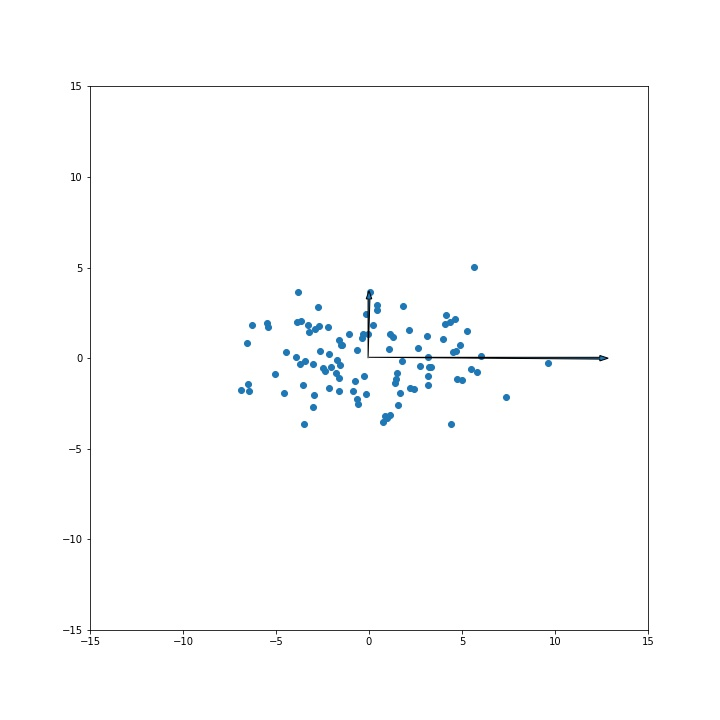
\includegraphics[width=8cm]{HW03_prob3e.jpg}
\end{multicols}



\newpage
%%%%%%%%%%%%%%%%%%%%%%%%%%%%%%%%%% PROBLEM 4 %%%%%%%%%%%%%%%%%%%%%%%%%%%%%%%%%%
\section*{Problem 4}

Let $X_1, ... X_n \in \mathbb{R}^{d}$ be draw independently from multivariate normal distribution $\mathcal{N}(\mu,\Sigma)$.

\subsection*{\textit{a.})}

We can express the likelihood function of choosing $X_1,...X_n$ as
$$ \mathcal{L} = \prod_{i=1}^n{P(X_i)}, $$
and where $P(X_i)$ is given by the normal distribution such that
$$ P(X_i) = \frac{1}{\sqrt{(2\pi)^d|\Sigma|}}e^{-\frac{1}{2}(X_i-\mu)^T\Sigma^{-1}(X_i-\mu)}.$$

Then, taking the natural logarithm of the likelihood function we can express the log-likelihood function as
$$ \ell = \ln\left(\prod_{i=1}^n{P(X_i)}\right) = \sum_{i=1}^n{\ln P(X_i)} $$
$$ \ell = \sum_{i=1}^n{\ln \left(\frac{1}{\sqrt{(2\pi)^d|\Sigma|}}e^{-\frac{1}{2}(X_i-\mu)^T\Sigma^{-1}(X_i-\mu)}\right)} $$
$$ \ell = \sum_{i=1}^n{\ln \left(\frac{1}{\sqrt{(2\pi)^d|\Sigma|}}\right)} + \sum_{i=1}^n{\ln \left(e^{-\frac{1}{2}(X_i-\mu)^T\Sigma^{-1}(X_i-\mu)}\right)} $$
$$ \ell = \sum_{i=1}^n{-\frac{1}{2}(X_i-\mu)^T\Sigma^{-1}(X_i-\mu)} - \sum_{i=1}^n{\frac{1}{2} \ln \left((2\pi)^d|\Sigma|\right)} $$
$$ \ell = -\frac{1}{2}\left(\sum_{i=1}^n{(X_i-\mu)^T\Sigma^{-1}(X_i-\mu)} + \sum_{i=1}^n{\ln (2\pi)^d} + \sum_{i=1}^n{\ln |\Sigma|}\right) $$
$$ \ell = -\frac{1}{2}\left(\sum_{i=1}^n{(X_i-\mu)^T\Sigma^{-1}(X_i-\mu)} + nd\,{\ln (2\pi)} + n\ln |\Sigma| \right) $$

To calculate the maximum likelihood estimate for $\mu$ (actually maximizing $\hat{\mu}$, as we may only estimate the mean of the distribution), we take the gradient with respect to $\mu$ and set it equal to zero.
$$ \nabla_{\mu}\ell = \nabla_{\mu}\left( -\frac{1}{2}\left(\sum_{i=1}^n{(X_i-\mu)^T\Sigma^{-1}(X_i-\mu)} + nd\,{\ln (2\pi)} + n\ln |\Sigma| \right) \right) $$
$$ \nabla_{\mu}\ell = -\frac{1}{2}\nabla_{\mu}\left(\sum_{i=1}^n{(X_i-\mu)^T\Sigma^{-1}(X_i-\mu)} \right) $$
$$ \nabla_{\mu}\ell = -\frac{1}{2}\sum_{i=1}^n{\nabla_{\mu}\left((X_i-\mu)^T\Sigma^{-1}(X_i-\mu)\right)} $$
In the previous homework (problem 2b.) we showed that if $A$ is square and symmetric, then $ \nabla_x(x^TAx) = 2Ax $. Applying the chain rule, if $x$ is a function of $y$, then we can state that $\nabla_y(x^TAx) = \nabla_x(x^TAx)\nabla_y x = 2Ax\, \nabla_y x$. If we let $x = (X_i-\mu)$ and $\Sigma^{-1} = A$, then we find 
$$ \nabla_{\mu}\ell = -\frac{1}{2}\sum_{i=1}^n{\nabla_{\mu}(x^TAx)} = -\frac{1}{2}\sum_{i=1}^n{\nabla_{x}(x^TAx)\,\nabla_{\mu}x} $$
$$ \nabla_{\mu}\ell = -\frac{1}{2}\sum_{i=1}^n{2Ax\,\nabla_{\mu}x} $$
$$ \nabla_{\mu}\ell = -\sum_{i=1}^n{\Sigma^{-1} (X_i-\mu)\,\nabla_{\mu}(X_i-\mu)} $$
$$ \nabla_{\mu}\ell = \sum_{i=1}^n{\Sigma^{-1} (X_i-\mu)} $$
$$ \nabla_{\mu}\ell = \sum_{i=1}^n{\Sigma^{-1}X_i}-\sum_{i=1}^n{\Sigma^{-1}\mu} $$
$$ \nabla_{\mu}\ell = \Sigma^{-1}\sum_{i=1}^n{X_i}-n\Sigma^{-1}\mu $$
Setting $\nabla_{\mu}\ell = 0,$
$$ 0 = \Sigma^{-1}\sum_{i=1}^n{X_i}-n\Sigma^{-1}\mu $$
$$ n\Sigma^{-1}\mu = \Sigma^{-1}\sum_{i=1}^n{X_i} $$
$$\boxed{ \hat{\mu} = \frac{1}{n}\sum_{i=1}^n{X_i} }$$

To calculate the maximum likelihood estimate for $\hat{\sigma}_j$ we take the partial derivative with respect to $\sigma_j$ and set it equal to zero (note that here I have redefined $\hat{\sigma}_i$---as given in the problem---as $\hat{\sigma}_j$ to avoid confusing counting indices for $n$ and $d$).
$$ \frac{\partial \ell}{\partial \sigma_j} = \frac{\partial}{\partial \sigma_j}\left( -\frac{1}{2}\left(\sum_{i=1}^n{(X_i-\mu)^T\Sigma^{-1}(X_i-\mu)} + nd\,{\ln (2\pi)} + n\ln |\Sigma| \right) \right) $$
$$ \frac{\partial \ell}{\partial \sigma_j} =  -\frac{1}{2} \frac{\partial}{\partial \sigma_j}\left(\sum_{i=1}^n{(X_i-\mu)^T\Sigma^{-1}(X_i-\mu)} + n\ln |\Sigma| \right) $$
We are given that the distribution has unknown diagonal covariance matrix, where the $j^{\text{th}}$ element of the diagonal, $\Sigma_{jj} = \sigma_j^2$. From this, we can directly conclude that the inverse of the covariance matrix, $\Sigma^{-1}$,  is also a diagonal matrix with diagonal elements $(\Sigma^{-1})_{jj} = 1/\sigma_{j}^2$. With this form, we can simplify the matrix product in the summation term above to yield
$$ \frac{\partial \ell}{\partial \sigma_j} =  -\frac{1}{2} \frac{\partial}{\partial \sigma_j}\left(\sum_{i=1}^n{\sum_{j=1}^d{\frac{|X_{ij}-\mu|^2}{\sigma_{j}^2}}} + n\ln |\Sigma| \right) $$
Furthermore, for diagonal matrices, we can express the determinant as the product of the diagonal elements.
$$ \frac{\partial \ell}{\partial \sigma_j} =  -\frac{1}{2} \frac{\partial}{\partial \sigma_j}\left(\sum_{i=1}^n{\sum_{j=1}^d{\frac{|X_{ij}-\mu_j|^2}{\sigma_{j}^2}}} + n\ln \left(\prod_{j=1}^d{\sigma_j^2}\right) \right)$$
$$ \frac{\partial \ell}{\partial \sigma_j} =  -\frac{1}{2} \frac{\partial}{\partial \sigma_j}\left(\sum_{i=1}^n{\sum_{j=1}^d{\frac{|X_{ij}-\mu_j|^2}{\sigma_{j}^2}}} + n\sum_{j=1}^d{\ln \sigma_j^2} \right)$$
$$ \frac{\partial \ell}{\partial \sigma_j} =  -\frac{1}{2}\left[\frac{\partial}{\partial \sigma_j}\left(\sum_{i=1}^n{\sum_{j=1}^d{\frac{|X_{ij}-\mu_j|^2}{\sigma_{j}^2}}}\right)+  \frac{\partial}{\partial \sigma_j}\left( n\sum_{j=1}^d{\ln \sigma_j^2} \right)\right]$$
$$ \frac{\partial \ell}{\partial \sigma_j} =  -\frac{1}{2}\left[\sum_{i=1}^n{\frac{\partial}{\partial \sigma_j}\left(\sum_{j=1}^d{\frac{|X_{ij}-\mu_j|^2}{\sigma_{j}^2}}\right)}+  n\frac{\partial}{\partial \sigma_j}\left( \sum_{j=1}^d{\ln \sigma_j^2} \right)\right]$$
$$ \frac{\partial \ell}{\partial \sigma_j} =  -\frac{1}{2}\left[\sum_{i=1}^n{\frac{\partial}{\partial \sigma_j}\left(\frac{|X_{ij}-\mu_j|^2}{\sigma_{j}^2}\right)}+  \frac{\partial}{\partial \sigma_j}\left( \ln \sigma_j^2 \right)\right]$$
$$ \frac{\partial \ell}{\partial \sigma_j} =  -\frac{1}{2}\left[\sum_{i=1}^n{|X_{ij}-\mu_j|^2\frac{\partial}{\partial \sigma_j}\left(\frac{1}{\sigma_{j}^2}\right)}+  2n\frac{\partial}{\partial \sigma_j} \ln (\sigma_j)\right]$$
$$ \frac{\partial \ell}{\partial \sigma_j} =  -\frac{1}{2}\left[\sum_{i=1}^n{|X_{ij}-\mu_j|^2\left(\frac{-2}{\sigma_{j}^3}\right)}+  2n\left(\frac{1}{\sigma_j}\right)\right]$$
$$ \frac{\partial \ell}{\partial \sigma_j} =  \sum_{i=1}^n{\left(\frac{|X_{ij}-\mu_j|^2}{\sigma_{j}^3}\right)} - \left(\frac{n}{\sigma_j}\right)$$
Setting $\frac{\partial \ell}{\partial \sigma_j} = 0,$
$$ 0 =  \sum_{i=1}^n{\left(\frac{|X_{ij}-\mu_j|^2}{\sigma_{j}^3}\right)} - \left(\frac{n}{\sigma_j}\right)$$
$$ 0 =  \sum_{i=1}^n{\left(\frac{|X_{ij}-\mu_j|^2}{\sigma_{j}^3}\right)} - \left(\frac{n\sigma_j^2}{\sigma_j^3}\right)$$
$$ 0 =  \sum_{i=1}^n{|X_{ij}-\mu_j|^2} - n\sigma_j^2 $$
$$ n\sigma_j^2 =  \sum_{i=1}^n{|X_{ij}-\mu_j|^2} $$
$$ \hat{\sigma}_j =  \sqrt{\frac{1}{n}\sum_{i=1}^n{|X_{ij}-\mu_j|^2}} $$
If we let $\mu_j = \hat{\mu}_j = \frac{1}{n}\sum_{i=1}^n{X_{ij}}$, then
$$\boxed{ \hat{\sigma}_j =  \sqrt{\frac{1}{n}\sum_{i=1}^n{\left|X_{ij}-\frac{1}{n}\sum_{i=1}^n{X_{ij}}\right|^2}} }$$



\subsection*{\textit{b.})}

Now the normal distribution has a known covariance matrix $\Sigma$, and an unknown mean $A\mu$. $\Sigma$ and $A$ are known $d \times d$ matrices, and $A$ is invertible. The multivariate normal distribution is given by
$$ \mathcal{N}(A\mu,\Sigma) = \frac{1}{\sqrt{(2\pi)^d|\Sigma|}}e^{-\frac{1}{2}(X_i-A\mu)^T\Sigma^{-1}(X_i-A\mu)} ,$$
the likelihood function is again given by
$$ \mathcal{L} = \prod_{i=1}^n{P(X_i)}, $$
and the log-likelihood function is given by
$$ \ell = \ln\left(\prod_{i=1}^n{P(X_i)}\right) = \sum_{i=1}^n{\ln P(X_i)}. $$
With the normal distribution as the probability density function for a given $X_i$, we have
$$ \ell = \sum_{i=1}^n{\ln \left(\frac{1}{\sqrt{(2\pi)^d|\Sigma|}}e^{-\frac{1}{2}(X_i-A\mu)^T\Sigma^{-1}(X_i-A\mu)}\right)}, $$
and following similar simplification steps to those used in part (a), we find
$$ \ell = -\frac{1}{2}\left(\sum_{i=1}^n{(X_i-A\mu)^T\Sigma^{-1}(X_i-A\mu)} + nd\,{\ln (2\pi)} + n\ln |\Sigma| \right) .$$
Again, we find the maximum likelihood estimate $\hat{\mu}$ for $\mu$ by maximizing the function with respect to $\mu$, namely where $\nabla_{\mu}\ell = 0$.
$$ \nabla_{\mu} \ell = \nabla_{\mu} \left(-\frac{1}{2}\left(\sum_{i=1}^n{(X_i-A\mu)^T\Sigma^{-1}(X_i-A\mu)} + nd\,{\ln (2\pi)} + n\ln |\Sigma| \right) \right) $$
$$ \nabla_{\mu} \ell = -\frac{1}{2} \sum_{i=1}^n{\nabla_{\mu} \left((X_i-A\mu)^T\Sigma^{-1}(X_i-A\mu)\right)} $$
$$ \nabla_{\mu} \ell = -\frac{1}{2} \sum_{i=1}^n{\nabla_{\mu} \left((X_i^T-(A\mu)^T)(\Sigma^{-1}X_i-\Sigma^{-1}A\mu)\right)} $$
$$ \nabla_{\mu} \ell = -\frac{1}{2} \sum_{i=1}^n{\nabla_{\mu} \left[(X_i^T\Sigma^{-1}X_i-(A\mu)^T\Sigma^{-1}X_i - X_i^T\Sigma^{-1}A\mu + (A\mu)^T\Sigma^{-1}A\mu)\right]} $$
$$ \nabla_{\mu} \ell = -\frac{1}{2} \sum_{i=1}^n{\left[-\nabla_{\mu}(\mu^TA^T\Sigma^{-1}X_i)- \nabla_{\mu}(X_i^T\Sigma^{-1}A\mu) + \nabla_{\mu}(\mu^TA^T\Sigma^{-1}A\mu)\right]} $$
Now, let $b = A^T\Sigma^{-1}X_i$ and $B = A^T\Sigma^{-1}A$, then
$$ \nabla_{\mu} \ell = -\frac{1}{2} \sum_{i=1}^n{\left[-\nabla_{\mu}(\mu^Tb)- \nabla_{\mu}(b^T\mu) + \nabla_{\mu}(\mu^TB\mu)\right]} $$
From the previous homework (problem 2a.) we showed that $\nabla_{\mu}(b^T\mu) = b$. Using a similar procedure, it can also be shown that $\nabla_{\mu}(\mu^Tb) = b$. Also in the previous homework (problem 2b.), we showed that $\nabla_{\mu}{\mu^TB\mu} = (B + B^T)x$. Using these equivalences, we find
$$ \nabla_{\mu} \ell = -\frac{1}{2} \sum_{i=1}^n{\left[-b - b + (B+B^T)\mu \right]} $$
$$ \nabla_{\mu} \ell = \sum_{i=1}^n{\left[b - \frac{(B+B^T)}{2}\mu \right]} $$
Setting $ \nabla_{\mu} \ell = 0 $,
$$ 0 = \sum_{i=1}^n{\left[b - \frac{(B+B^T)}{2}\mu \right]} $$
$$ 0 = \sum_{i=1}^n{b} - \sum_{i=1}^n{\frac{(B+B^T)}{2}\mu} $$
$$ \sum_{i=1}^n{\frac{(B+B^T)}{2}\mu} = \sum_{i=1}^n{b} $$
$$ \mu n \frac{(B+B^T)}{2} = \sum_{i=1}^n{b} $$
$$ \mu = \frac{2\sum_{i=1}^n{b}}{n(B+B^T)} $$
$$ \mu = \frac{2\sum_{i=1}^n{A^T\Sigma^{-1}X_i}}{n(A^T\Sigma^{-1}A+(A^T\Sigma^{-1}A)^T)} $$
Since covariance matrices are by definition symmetric, their inverses are also symmetric, and 
$$ \mu = \frac{2\sum_{i=1}^n{A^T\Sigma^{-1}X_i}}{n(A^T\Sigma^{-1}A+A^T\Sigma^{-1}A)} = \frac{2A^T\Sigma^{-1}\sum_{i=1}^n{X_i}}{2nA^T\Sigma^{-1}A} $$
$$ \mu = \frac{\sum_{i=1}^n{X_i}}{nA} $$
$$\boxed{ \hat{\mu} = \frac{1}{2} A^{-1} \sum_{i=1}^n{X_i} }$$



\newpage
%%%%%%%%%%%%%%%%%%%%%%%%%%%%%%%%%% PROBLEM 5 %%%%%%%%%%%%%%%%%%%%%%%%%%%%%%%%%%
\section*{Problem 5}

\subsection*{\textit{a.})}

Any matrix is not invertible if and only if it's determinant is zero. Therefore, $\hat{\Sigma}$ is not invertible if and only if $|\hat{\Sigma}| = 0$. From this, we can use the property that the determinant of a square matrix is equal to the product of the eigenvalues of that matrix to deduce that if $|\hat{\Sigma}| = 0$, then at least one of the eigenvalues of $\hat{\Sigma}$ must be zero. 

Geometrically, a matrix with $n$ zero eigenvalues represents a transformation from a $d$-dimensional space to a $(d-n)$-dimensional space, with the dimensions corresponding to the zero eigenvalues vanishing.

This situation, in which a $d$-dimensional space collapses to a $(d-n)$-dimensional space could be visualized by a data set, in our case random values of $X_i$ pulled from the multivariate normal distribution, in which the points have no variance in $n$-dimensions. Geometrically, these points would fall on the same hyperplane in $(d-n+1)$-dimensional space.


\subsection*{\textit{b.})}

Given that at least one eigenvalue of a singular covariance matrix must be zero, we can deduce that there is no variance in that parameter. Without variance, our machine-learning algorithm will have no ability to use that parameter as a discriminator. A workaround could be that we eliminate all variables with zero variance from influencing our covariance matrix. In the equation for determining the covariance matrix estimator, this is achieved by removing the $j^{\text{th}}$ row and column $\{j:1,...,d\}$ if $(X_{ij} - \mu_j ) =0 \;\; \forall i \in n$. 


\subsection*{\textit{c.})}

Maximizing $f(x)$ for vectors $|x| = 1$ requires maximizing the argument of the exponential. We are told that $\mu = 0$, so we are looking for the maximum of 
$$ g(x) = x^T\Sigma^{-1}x, \;\; |x|= 1 $$
In the previous homework (problem 4a.) we proved that $\lambda_{\text{max}}(A) = \max_{|x|=1}{x^TAx}$. From this, we can state
$$ \max_{|x|=1}{g(x)} = \max_{|x|=1}{x^T\Sigma^{-1}x} = \lambda_{\text{max}}(\Sigma^{-1}) $$
We can show that the vector $x$ which satisfies this equation is \uline{the eigenvector corresponding to the maximum eigenvalue of $\Sigma^{-1}$}:
$$ xx^T\Sigma^{-1}x = x\lambda_{\text{max}}(\Sigma^{-1}), \; xx^T = 1$$
$$ \Sigma^{-1}x = \lambda_{\text{max}}(\Sigma^{-1})x $$

Using the same procedure to calculate the minimum, and again using our results from the previous homework (problem 4b.) we can state
$$ \min_{|x|=1}{g(x)} = \min_{|x|=1}{x^T\Sigma^{-1}x} = \lambda_{\text{min}}(\Sigma^{-1}) $$
and 
$$ xx^T\Sigma^{-1}x = x\lambda_{\text{min}}(\Sigma^{-1}), \; xx^T = 1$$
$$ \Sigma^{-1}x = \lambda_{\text{min}}(\Sigma^{-1})x $$
The vector $x$ with $|x|=1$ which gives the minimum of $f(x)$ is \uline{the eigenvector correspondingto the minimum eigenvalue of $\Sigma^{-1}$}.





\newpage
%%%%%%%%%%%%%%%%%%%%%%%%%%%%%%%%%% PROBLEM 6 %%%%%%%%%%%%%%%%%%%%%%%%%%%%%%%%%%
\section*{Problem 6}

\subsection*{\textit{a.})}

Mean and covariance matrices were calculated, see Appendix for code, and (b) for visualization.


\subsection*{\textit{b.})}

\includegraphics[width = 18cm]{VisualCovMatrices}


\subsection*{\textit{c.})}
\begin{multicols}{2}
\subsubsection*{(i) LDA}

Test errors plotted against number of sample points: \\
\small(note that there seems to be large variation among training sets of relatively few samples)\\
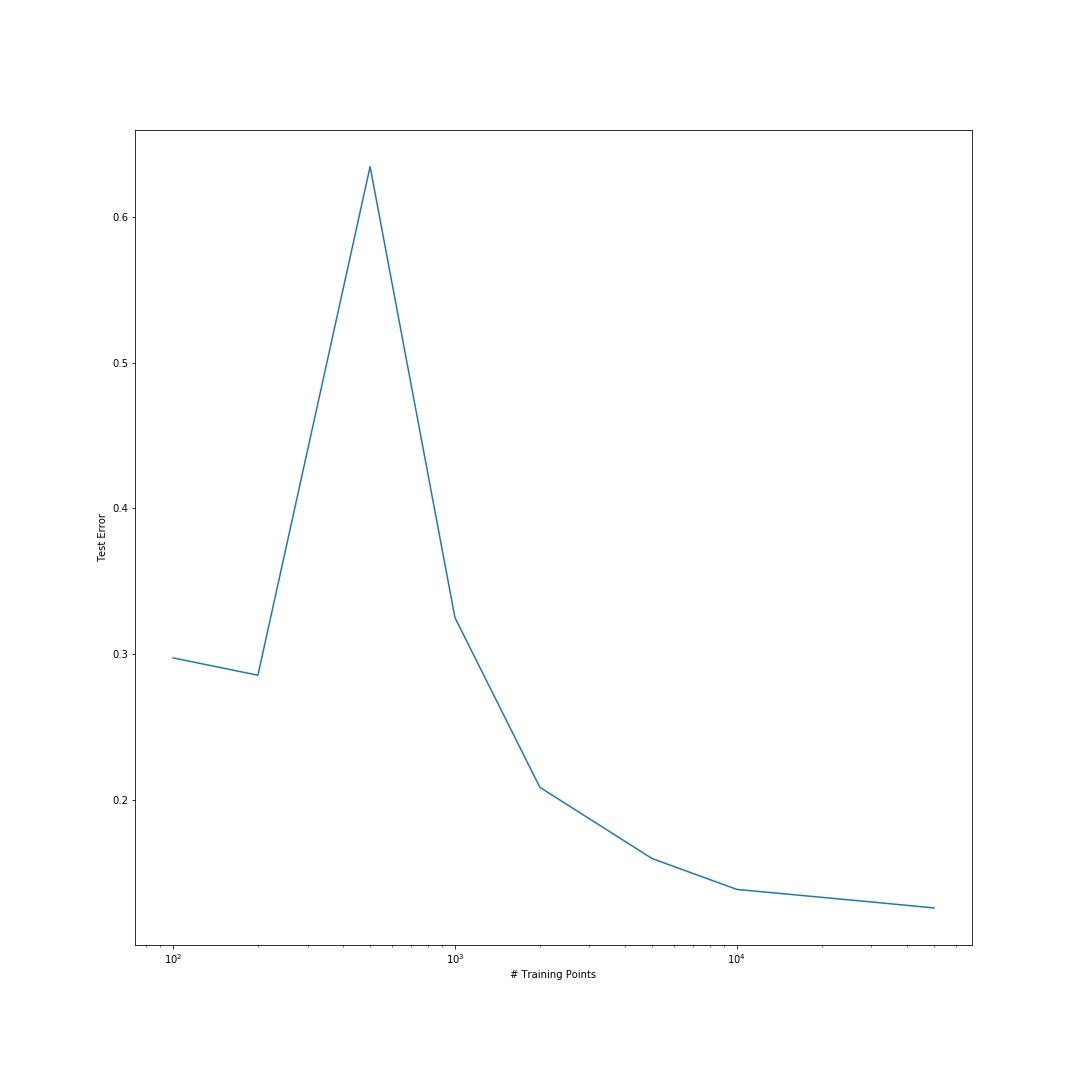
\includegraphics[width=8cm]{LDA_errors}
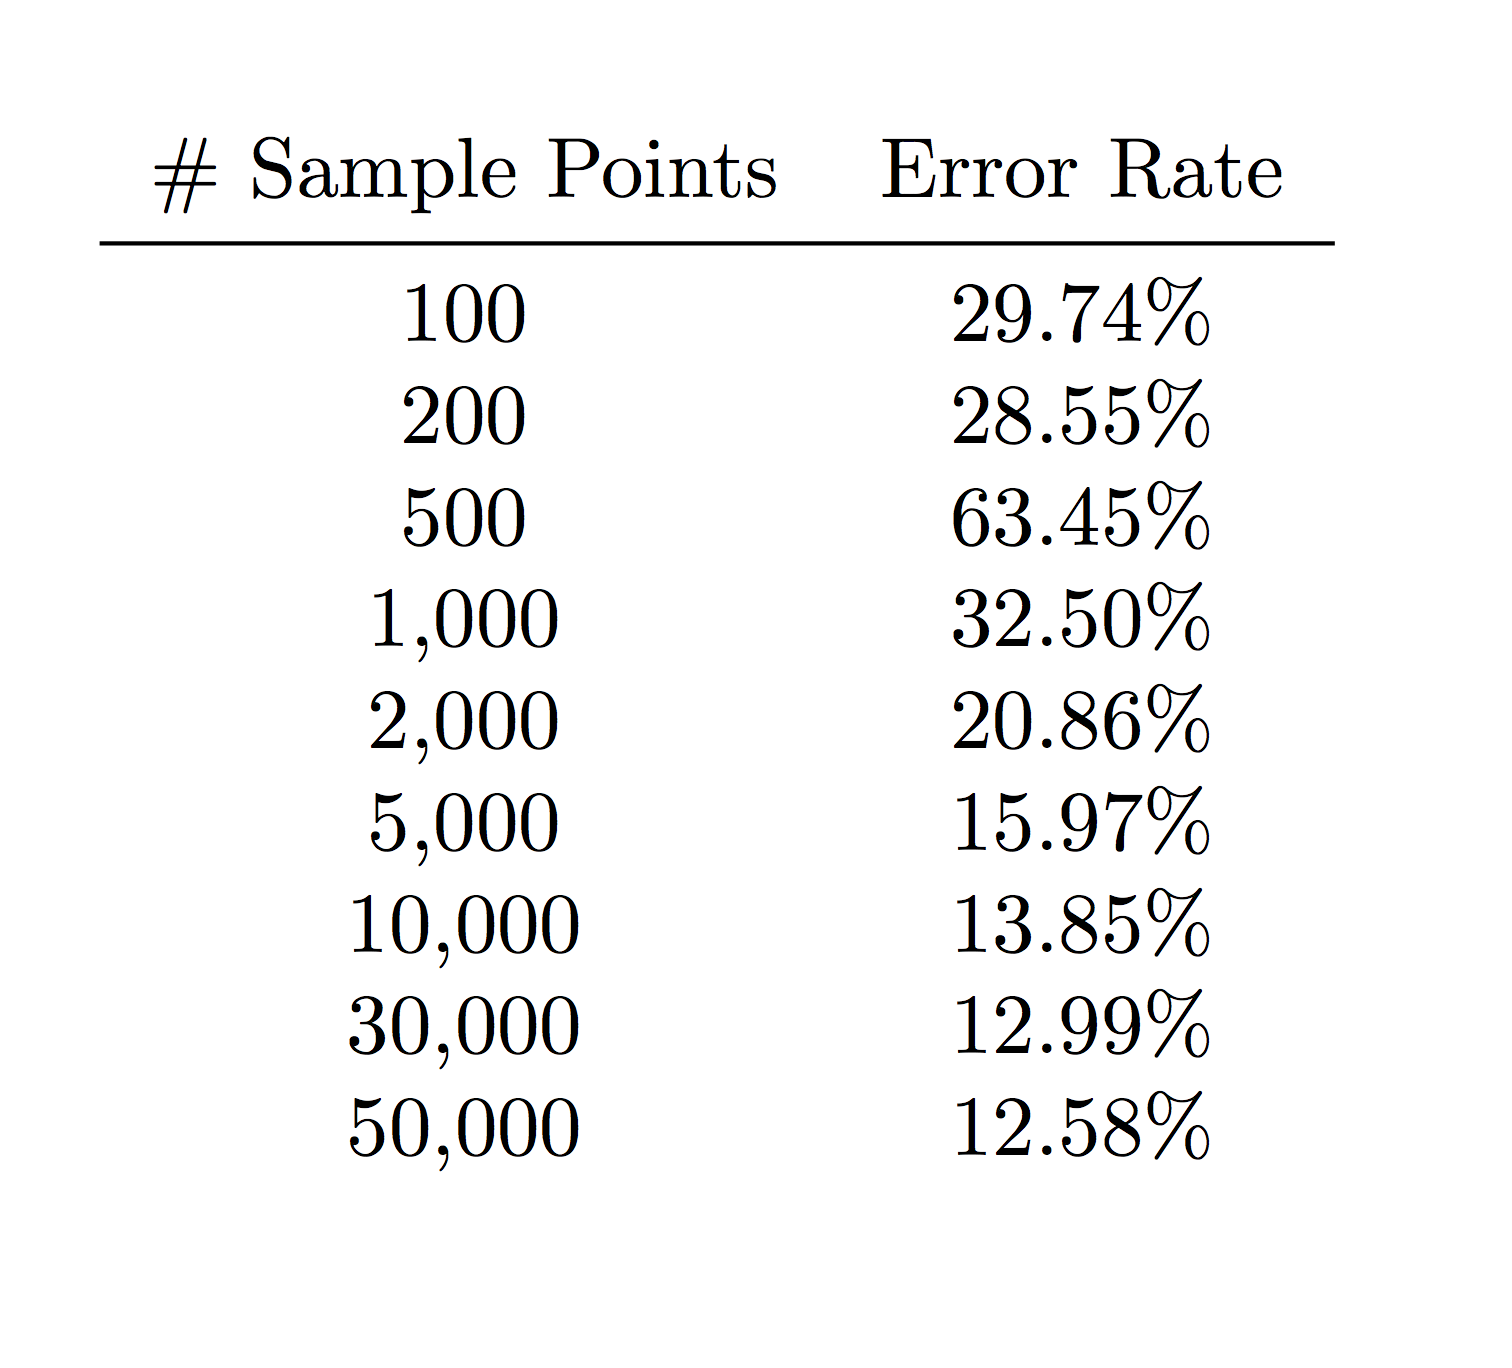
\includegraphics[width=8cm]{LDA_errorTable}

\columnbreak
\subsubsection*{(ii) QDA}


(code included; no plot as I was unsuccessful in resolving singular covariance matrix issue before due date)\\



\end{multicols}



\end{document}





